\chapter{Implementierung der Betriebssoftware}
Die Betriebssoftware wurde, wie in der Aufgabenstellung festgelegt in C geschrieben.
Hierbei fiel die Wahl auf den Standard C99, der mit einigen sprachlichen
Aktualisierungen gegenüber C89 aufwarten kann. Als Compiler wurde eine Version der
GNU Compiler Collection (GCC) mit einem Backend für AVR-kompatiblen Assembler benutzt.
Außer der C Standard Library und der AVR IO Library besitzt die Software keine externen
Abhängigkeiten im Code.
\section{Die Hauptschleife}
Die Hauptschleife ist in dieser Implementierung eine Endlosschleife, da die Beendigung dieser
Schleife dazu führen würde, dass das System nicht mehr reagiert.
Wie in Abb. \ref{main_loop} zu sehen ist, werden in der Hauptschleife vier wichtige Funktionen
aufgerufen.
\subsection{process\_orders()}
Die process\_\-orders()\--Funktion bearbeitet die Befehle, die bereits in der Queue sind. Dafür holt
sich die Funktion den aktuellen Befehl von der Queue. Falls es solch einen Befehl gibt ruft die
Funktion eine Verteilerfunktion auf. Diese wiederum ruft die zugehörige Befehlsfunktion auf, indem
die untersten vier Bits des ersten Befehlsbytes als Index für eine Call-Table benutzt werden (siehe
Abb. \ref{dispatch_function}).\\
\begin{figure}[htb]
 \centering
 \scalebox{0.6}{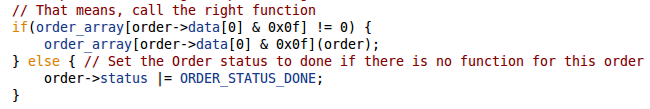
\includegraphics{pictures/dispatch_function.png}}
 \caption{\label{dispatch_function}Die Verteilerfunktion}
\end{figure}
Falls kein Befehl vorliegt oder die Queue angehalten wurde, ruft die process\_\-orders()-Funktion die
Funktion zum aktiven Bremsen auf. Das aktive Bremsen wird in Kapitel \ref{chapter_abs} behandelt.
\subsection{lcd\_update\_screen()}
In dem Fall, dass ein LCD angeschlossen ist, können dort Informationen ausgegeben werden. Ob ein LCD
angeschlossen ist wird über die Stellung eines DIP-Schalters auf der Platine geregelt.\\
Da das synchrone Aktualisieren des LCD sehr viel Zeit benötigt (vgl. Kapitel \ref{chapter_lcd_problem}), wird
während dieser Funktion maximal ein Zeichen an das LCD geschickt. Dies wird erreicht indem das Busy-Flag,
welches signalisiert, dass das LCD noch beschäftigt ist, abgefragt wird. Falls es nicht gesetzt ist und
es noch Daten zum aktualisieren gibt, wird das nächste Zeichen an das LCD gesendet.\\
Auf dem LCD werden die Versionsnummer der Betriebssoftware, der Status einiger system-weiter Variablen und
der aktuelle ausgeführte Befehl angezeigt. Falls nun ein Befehl bearbeitet wird, der länger als einen
Schleifendurchlauf benötigt (das sind z.B. alle Fahr-Befehle), ruft die lcd\_\-update\_\-screen()-Funktion
die lcd\_\-update\_\-info()-Funktion auf, die diese Informationen in einem Puffer konstruiert. Nach und nach
gibt die lcd\_\-update\_\-screen()-Funktion den Inhalt dieses Puffer an das LCD weiter.\\
Befehle die innerhalb eines Hauptschleifendurchlaufs abgearbeitet sind werden nicht ausgegeben und
generieren auch keinen Aufruf von lcd\_\-update\_\-info(). Dies ist nötig, da diese Befehle zu schnell abgearbeitet
werden. Es können vier bis fünf dieser Befehle abgearbeitet werden, bevor das LCD auch nur einmal vollständig
aktualisiert werden kann.
\subsection{parser\_update()}
Der Parser ist dafür zuständig aus den Bytes, die über I2C oder UART gelesen werden, Befehle in Form von
order\_t-Strukturen zu erstellen. Die parser\_\-update()-Funktion fragt beim IO-Modul nach, wie viele Bytes
zum Abholen bereit stehen. Diese werden dann geholt und an die Funktion parser\_\-add\_\-byte() übergeben.\\
Diese parser\_\-add\_\-byte()-Funktion fügt das Byte an die korrekte Stelle im Puffer ein. Wenn ein Befehl
komplett ist, was mit der parser\_\-order\_\-complete()-Funktion überprüft wird, gilt der Befehl als fertig und
alle weiteren Bytes, die hinzugefügt werden, landen in einer neuen order\_t-Struktur.\\
Damit erkannt werden kann, wann ein Befehl zu ende ist benutzt die parser\_\-order\_\-complete()-Funktion
die bytes\_\-needed()-Funktion, in der fest codiert ist, welcher Befehlscode mit welchen Optionen wie viele
Bytes benötigt. Dies ist auch eine der Stellen, die angepasst werden müssen, wenn ein neuer Befehl hinzugefügt
wird, oder bestehende verändert werden.
\subsection{queue\_update()\label{chapter_queue_update}}
Diese Funktion führt Wartungsarbeiten an der Befehlswarteschlange (Queue) durch. Dies beinhaltet neue
Befehle beim Parser-Modul abzuholen und diese korrekt einzureihen. Es gibt zwei Möglichkeiten, wie die Queue
diese neuen Befehle einreihen kann. Zum einen als normale Befehle, diese werden einer nach dem anderen abgearbeitet,
zum anderen als priorisierte Befehl. Es kann nur ein priorisierter Befehl in der Queue sein. Diese Befehle werden
umgehend in der nächsten Haupt\-schleifen\-iteration ausgeführt. In die Kategorie der priorisierten Befehle fallen
alle Queue-Kontroll-Befehle, wie z.B. pausieren, löschen, aktuellen Befehl verwerfen, etc. (vgl. Kapitel \ref{chapter_protokoll}).
\section{Das Aktive Brems-System (ABS)\label{chapter_abs}}
Das aktive Bremssystem bewirkt, dass die Räder versuchen ihre Position nicht zu verlassen. Dies wird realisiert indem
eine Referenz-Position für jedes Rad gespeichert wird. Während der Hauptschleife wird nun die tatsächliche Position mit
der Referenz-Position verglichen. In dem Fall, dass diese Positionen nicht übereinstimmen, werden die Motoren mit einer
einstellbaren Geschwindigkeit betrieben, um die Räder wieder auf die Referenz-Position zu bringen.\\
Die Referenz-Positionen werden an drei verschiedenen Stellen im Code gesetzt. Zum einen in der process\_\-orders()-Funktion
in der Hauptschleife, wenn der aktuelle Befehl beendet wurde, zum anderen in den Fahr-Befehls-Funktionen, falls ein Rad
früher als das andere seine Stopp-Bedingung erreicht hat.\\
Das ABS kann vom Benutzer während das System läuft, angepasst werden. So kann man die Geschwindigkeit ändern, mit der
die Motoren die Positions-Differenz ausgleichen. Außerdem kann man Teile des ABS deaktivieren oder auch wieder reaktivieren
sowie das gesamte ABS abschalten, bzw. wieder anschalten. Damit kann der Benutzer das ABS an seine Wünsche anpassen.
\section{Befehle: Struktur und Funktionen}
Die Struktur (Abb. \ref{order_type}), die einen Befehl im System repräsentiert, besteht hauptsächlich aus einem Array, in dem die eigentlichen Daten
gespeichert sind, und einem Status-Byte, in dem Statusinformationen in Form von Flags gespeichert werden.
\begin{figure}[htb]
 \centering
 \scalebox{0.6}{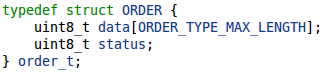
\includegraphics{pictures/order_t.png}}
 \caption{\label{order_type}Befehlsstruktur}
\end{figure}
Das erste Byte dieses Arrays ist das Typ-Byte, das die Art des Befehls und die zugehörigen Optionen spezifiziert. Der
Befehlscode (die unteren vier Bits des Typ-Bytes) 0 ist für zukünftige Erweiterungen Reserviert, die mehr als ein Typ-Byte
benötigen. Des weiteren sind die Befehlscodes 1 bis 6 durch diese Arbeit bereits definiert und mit Funktionalität erfüllt.
Die Befehlscodes 7 bis 15 sind noch nicht definiert und können für zukünftige Erweiterungen benutzt werden, die mit einem
Typ-Byte auskommen.\\
Alle auf das Typ-Byte (oder die Typ-Bytes im Falle des Befehlscodes 0) folgenden Bytes sind Parameter. Die Anzahl und Länge
dieser hängt von der Spezifikation des Befehls ab. Grundsätzlich gilt aber, dass bei Parametern, mit mehr als ein Byte Länge,
zuerst das höchstwertige Byte im Array gespeichert wird, dann absteigend bis zum niederwertigsten Byte.\\
Oft benutze Aktionen bezüglich der Befehlsstruktur wurden zusammengefasst (siehe Abb. \ref{order_init} und \ref{order_copy}).
Vor der Untersuchung des Laufzeitverhaltens und der damit einhergehenden Optimierungen, wurden diese beiden Funktionen
durch for-Schleifen implementiert, was sich aber als langsamer als die Standard C Funktionen memset() und memcpy()
herausstellte.
\begin{figure}[htb]
 \centering
 \scalebox{0.6}{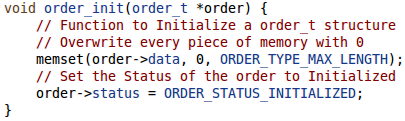
\includegraphics{pictures/order_init.png}}
 \caption{\label{order_init}order\_init()-Funktion}
\end{figure}
\begin{figure}[htb]
 \centering
 \scalebox{0.6}{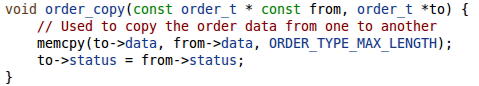
\includegraphics{pictures/order_copy.png}}
 \caption{\label{order_copy}order\_copy()-Funktion}
\end{figure}
\section{Datenpfad von Befehlen}
Befehle werden entweder über die UART oder die I2C Schnittstelle byteweise empfangen. Diese Schnittstellen werden über
Interrupt Service Routinen bearbeitet, um zeitnah auf eingehende Daten zu reagieren, da diese Übertragung die größte
Latenz-Quelle darstellt (I2C: ca. 270 \textmu{}s pro Byte; UART: ca 139 /textmu{}s pro Byte). In diesen Interrupt Service Routinen wird
das empfangene Byte in den Eingangspuffer gelegt. Wenn die Hauptschleife wieder die parser\_\-update()-Funktion erreicht,
wird die bisher empfangene Bytes abgeholt und in der Parser-Puffer abgelegt, um aus den Bytes order\_t Struktur Instanzen
zu generieren. Wenn der Befehl fertig im Parser vorliegt, ruft ihn queue\_\-update() ab und reiht ihn in die Warteschlange
ein (siehe Kapitel \ref{chapter_queue_update}). Von der Warteschlange holt sich die process\_\-orders()-Funktion den
aktuellen Befehl und führt die zugeordnete order\_function-Funktion solange aus, bis im Status-Byte (vgl. Abb. \ref{order_type})
das ORDER\_\-STATUS\_\-DONE Flag gesetzt wurde und entfernt diese dann aus der Warteschlange.\\
Falls der Befehl, der bearbeitet wird, eine Ausgabe von Daten bewirkt, wird in der entsprechenden order\_\-function-Funktion
die auszugebenden Daten in den Ausgabepuffer des IO-Framework angereiht. Dieses Framework wird dann, sobald möglich, diese Daten
über die ausgewählte Schnittstelle senden (bei UART wird sofort angefangen zu senden, bei I2C muss gewartet werden, bis die Daten
vom Benutzer abgerufen werden).
% Datenpfadbild
\section{Debug-Ausgaben \label{impl_debug}}
Das Problem mit Debug-Ausgaben ist, dass sie notwendig sind, insbesondere wenn die Benutzung eines üblichen Debuggers nicht
ohne weiteres möglich ist. Debug-Ausgaben benötigen entsprechenden Code, nicht nur um die Ausgaben überhaupt zu ermöglichen,
sonder auch an vielen Stellen im Code, um wirklich etwas zu bestimmten Zeitpunkten auszugeben. Diese Ausgaben, selbst wenn
sie nicht gemacht werden müssen, indem sie mit if-Statements umschlossen werden (siehe Abb. \ref{debug_trick}), verlangsamen
das gesamte System. Während der normalen Operation der Betriebssoftware im Praktikum, sind diese Ausgaben nicht nötig und für
die meisten Teilnehmer des Praktikums, nicht informativ. Damit die Ausgaben zum Zweck der Fehlerbehebung benutzt werden können,
muss der Benutzer eine entsprechende Kenntnisse des Codes vorweisen.\\
Aufgrund dieser fragwürdigen Hilfe, die diese Ausgaben einem durchschnittlichen Praktikanten bieten, und der negativen Auswirkung
der Ausgaben auf die Performance des Systems, wurde eine Prä-Prozessor Technik angewandt, die zusammen mit der eingestellten Stufe
der Code-Optimierung des Compilers diese beiden Probleme löst. Durch diese Technik werden die Debug-Ausgaben nur dann mitkompiliert,
wenn dem Compiler der Parameter -DDEBUG übergeben wird. Selbst dann ist es noch möglich mit einem DIP-Schalter auf der Platine
die Ausgaben auszuschalten, dann hat man aber immer noch die leichten negativen Auswirkungen auf die Performance. Normalerweise
wird die Betriebssoftware ohne diesen Parameter kompiliert. Das bedeutet, dass die Software neukompiliert werden muss, wenn
diese Debug-Ausgaben erwünscht sind.
\begin{figure}[htb]
 \centering
 \scalebox{0.5}{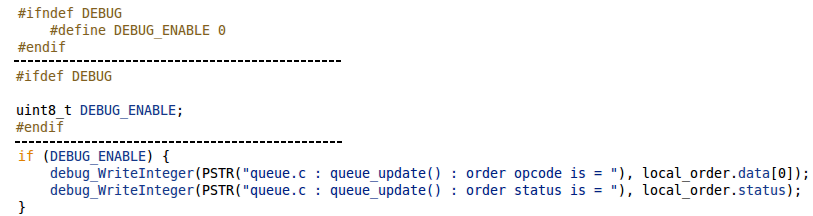
\includegraphics{pictures/debug_trick.png}}
 \caption{\label{debug_trick}Debug-Defines und die Verwendung im Code}
\end{figure}
\section{IO-Framework}
Das Ziel des IO-Frameworks war die Abstraktion der Ein- und Ausgabe von Daten von den zu Grunde liegenden Schnittstellen.
Die UART und die I2C Schnittstelle sind in der Benutzung sehr unterschiedlich. Statt überall im Code wo E/A stattfindet
jeweils für beide Schnittstellen Code einzufügen, wurde das IO-Framework als Zwischenschicht entwickelt. Es verfügt über sowohl
über einen Ausgabe- als auch über einen Eingabepuffer. Diese sind jeweils auf 256 Bytes festgelegt. Durch diese Definition
konnte das normale "Uberlaufverhalten der 8-Bit-Variablen ausgenutzt werden, um Modulo-Operationen zu ersetzen, welche
ungerechtfertigt viel Zeit in Anspruch nehmen.\\
Eine Besonderheit ist die Objekt-basierte Ausgabe von Daten. Ein Objekt hat mindestens ein Byte und maximal 256 Byte. Objekte
werden bei entweder komplett Übertragen oder gar nicht. Wenn ein Objekt nicht komplett übertragen werden konnte, wird bei der
nächsten Übertragen vom Anfang der Objektes wieder angefangen. Außerdem bewirkt die Ausgabe von Objekten bei Benutzung der I2C 
Schnittstelle, dass für jede Lese-Operation, die von der Praktikumsplatine eingeleitet wird, ein Objekt übermittelt wird.\\
E/A-Operationen geschehen nicht-blockend und gepuffert. Damit verbraucht die E/A nur Prozessor-zeit, wenn es nötig ist und
verschwendet diese nicht mit aktiven Warten.
\section{Unterstützende Bibliothek für die Praktikumsplatine}
